\chapter{General framework of \smtrat}
\label{chapter:generalframework}
\smtrat is a \Cpp library consisting of a collection of
SMT-compliant implementations of methods for solving non-linear real
and integer arithmetic (NRA/NIA) formulas, we refer to as modules. These modules can be 
combined to (1) a theory solver in order to extend the supported logics of an
existing SMT solver by NRA/NIA (see Figure~\ref{fig:frameworkb}) or (2) an SMT 
solver for NRA/NIA (see Figure~\ref{fig:frameworka}). The latter is 
especially intended to be a testing environment for the development 
of SMT-compliant implementations of further methods tackling NRA/NIA. Here,
the developer only needs to implement the given interfaces of an \smtrat 
module and does not need to care about parsing input files, transforming
formulas to conjunctive normal form or embedding a SAT solver in order
to solve the Boolean skeleton of the given formula. Instead, \smtrat
provides this and more features, such as lemma exchange and bound
extraction, which will be explained in following.

\begin{figure}[ht]
\caption{A snapshot of an \smtrat composition being an SMT solver for NRA.}
\begin{center}
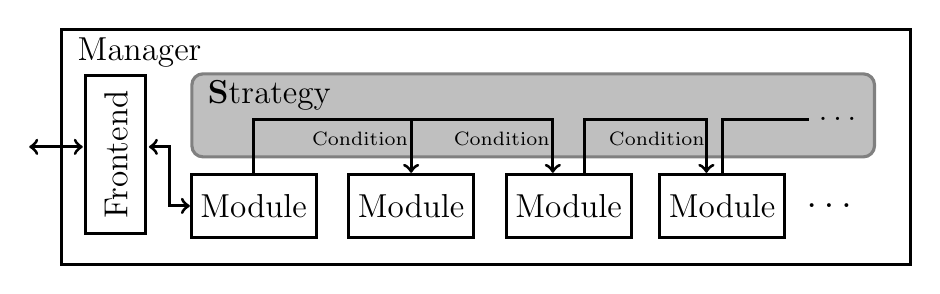
\begin{tikzpicture}[every node/.style={rectangle}, text centered, bend angle=15, line width=.4mm]
	\node[draw, minimum height=57pt, text width=15pt] (manager) at (-6.3, .2) {};
	\node[rotate=90] (managerText) at (-6.3, .2) {\large Frontend};
	\node[draw, minimum height=85pt, text width=300pt] (manager) at (-1.6, 0.3) {};
	\node[] (managerText) at (-6, 1.5) {\large Manager};
	\node[fill=lightgray,draw=gray, rounded corners, minimum height=30pt, text width=240pt] (strategy) at (-1,.7) {};
	\node[] (strategyText) at (-4.35, .95) {\large\textbf Strategy};
	\draw[<->] (-5.36,-.45) -- (-5.62,-.45) -- (-5.62,.3) -- (-5.88,.3);
	\draw[<->] (-6.72,.3) -- (-7.4,.3);
	\draw[->] (-4.55,-.03) -- (-4.55,.65) -- (-.75,.65) -- (-.75,-.03);
	\node[] (strategyText) at (-1.4, .4) {\scriptsize Condition};
	\draw[->] (-2.55,.65) -- (-2.55,-.03);
	\node[] (strategyText) at (-3.2, .4) {\scriptsize Condition};
	\draw[->] (-.35,-.03) -- (-0.35,.65) -- (1.2,.65) -- (1.2,-.03);
	\node[] (strategyText) at (.57, .4) {\scriptsize Condition};
	\draw (1.4,-.03) -- (1.4,.65) -- (2.5,.65);
	\node[] (dotsa) at (2.9,.65) {\large \ldots};
	\node[draw, minimum height=23pt] (moduleAText) at (-4.55, -.45) {\large Module};
	\node[draw, minimum height=23pt] (moduleBText) at (-2.55, -.45) {\large Module};
	\node[draw, minimum height=23pt] (moduleCText) at (-.55, -.45) {\large Module};
	\node[draw, minimum height=23pt] (moduleDText) at (1.4, -.45) {\large Module};
	\node[] (dotsc) at (2.8, -.45) {\Large \ldots};
\end{tikzpicture}%

\end{center}
\label{fig:frameworka}
\end{figure}

\begin{figure}[ht]
\caption{A snapshot of an \smtrat composition being a theory solver embedded in an SMT solver.}
\begin{center}
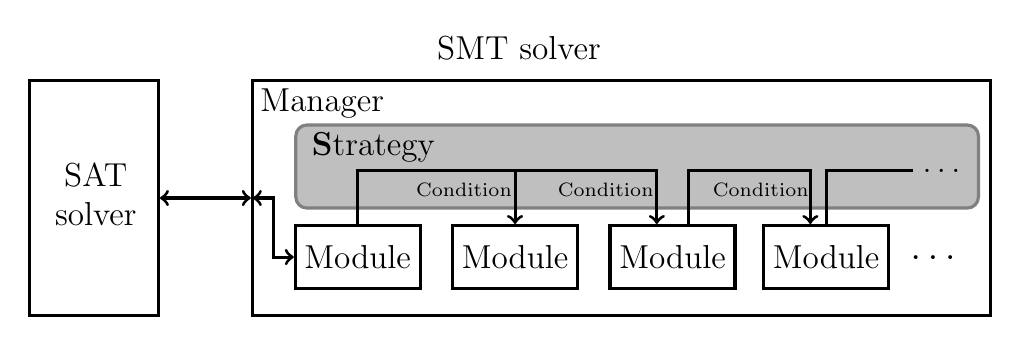
\begin{tikzpicture}[every node/.style={rectangle}, text centered, bend angle=15, scale=1, line width=.4mm]
	\node[] (smtsolver) at (-2.5, 2.2) {\large SMT solver};
	\node[draw, minimum height=85pt, text width=40pt] (satsolver) at (-7.9, 0.3) {\large\begin{tabular}{c}SAT \\ solver\end{tabular}};
	\node[draw, minimum height=85pt, text width=260pt] (manager) at (-1.2, 0.3) {};
	\node[] (managerText) at (-5, 1.5) {\large Manager};
	\node[fill=lightgray,draw=gray, rounded corners, minimum height=30pt, text width=240pt] (strategy) at (-1,.7) {};
	\node[] (strategyText) at (-4.35, .95) {\large\textbf Strategy};
	\draw[<->] (-5.36,-.45) -- (-5.62,-.45) -- (-5.62,.3) -- (-5.88,.3);
	\draw[->] (-4.55,-.03) -- (-4.55,.65) -- (-.75,.65) -- (-.75,-.03);
	\node[] (strategyText) at (-1.4, .4) {\scriptsize Condition};
	\draw[->] (-2.55,.65) -- (-2.55,-.03);
	\node[] (strategyText) at (-3.2, .4) {\scriptsize Condition};
	\draw[->] (-.35,-.03) -- (-0.35,.65) -- (1.2,.65) -- (1.2,-.03);
	\node[] (strategyText) at (.57, .4) {\scriptsize Condition};
	\draw (1.4,-.03) -- (1.4,.65) -- (2.5,.65);
	\node[] (dotsa) at (2.9,.65) {\large \ldots};
	\node[draw, minimum height=23pt] (moduleAText) at (-4.55, -.45) {\large Module};
	\node[draw, minimum height=23pt] (moduleBText) at (-2.55, -.45) {\large Module};
	\node[draw, minimum height=23pt] (moduleCText) at (-.55, -.45) {\large Module};
	\node[draw, minimum height=23pt] (moduleDText) at (1.4, -.45) {\large Module};
	\node[] (dotsc) at (2.8, -.45) {\Large \ldots};
	\path[<->] (satsolver.0) edge[] node[left] {} (manager.180);
\end{tikzpicture}

\end{center}
\label{fig:frameworkb}
\end{figure}

\smtrat defines three types of components: the \emph{manager}, the \emph{strategy} and, as already mentioned, \emph{modules}. 
In addition, a frontend (1) provides the interfaces to an extern SMT 
solver or (2) parses an input file to a non-linear real arithmetic 
formula, we denote in the following just as formula.
In this section we first describe the functionality of a module and,
then, show how the manager composes different modules according to a
strategy to a solver.

\section{The \moduleClass class.} A module $m$ contains a set of
formulas, called its \emph{set of received formulas} and denoted by 
$\Crcv(m)$. The main
procedure of a module  is \texttt{check()} and either decides
whether $\Crcv(m)$ is satisfiable or not returning \SAT or \UNSAT,
respectively, or returns \UNKNOWN. Note, that a set of formulas is
semantically defined by their conjunction. We can manipulate the set
of received formulas by adding (removing) formulas $\varphi$ to (from)
it with \texttt{add($\varphi$)} (\texttt{remove($\varphi$)}). Usually, 
$\Crcv(m)$ is only changed slightly between two consecutive 
\texttt{check()} calls, hence, the solver's performance can be significantly improved if the modules can
make use of the results of previous checks, that is they support
\emph{incrementality} and \emph{backtracking}. In case that the module
determines the unsatisfiability of $\Crcv(m)$, it is expected to compute
at least one preferably small \emph{infeasible subset} $\Cinf(m)\subseteq
\Crcv(m)$. Moreover, a module has the possibility to name lemmas, which
are formulas being tautologies, that is they hold for all assignments
of the variables occuring in them. These lemmas should encapsulate
information which can be extracted from a module's internal state and
propagated among other \smtrat modules. Furthermore, \smtrat provides
the feature that a module itself can ask other modules for the
satisfiability of a set of formulas, called its \emph{set
of passed formulas} denoted by $\Cpass(m)$, using the procedure \texttt{runBackends()} which
is controlled by the manager. 

\section{The \managerClass and the \strategyClass class} 
\label{sec:managerstrategy}
TODO: priorities in the strategy\newline 
\smtrat allows a user to decide how to compose the different procedures,
which are implemented in the modules. For this purpose we provide a GUI
where the user can create such a composition we call strategy. Further
explanation can be found in Chapter~\ref{chapter:composingats}. Here, 
it is enough to know that a \emph{strategy} is a directed tree $T:=(V, E)$ with a set $V$ of
(instances of) modules as nodes and $E\subseteq V\times \Omega\times V$,
where $\Omega$ is a set of conditions. The \emph{manager} contains the
strategy and the input formula $C_{input}$, either received by a prefexed solver
or parsed from an example file. Furthermore, it maintains the
allocation of modules as follows. 

Initially, the manager calls the method
\texttt{check()} of the module $m_r$ given by the root of
the strategy with $\Crcv(m_r) = C_{input}$ being the set of received formulas of this
module. Whenever a module $m\in V$ calls
\texttt{runBackends()}, with $\Cpass(m)$ being its set of passed
formulas, the manager calls \texttt{check()} of each module
$m'$ with \Crcv(m') = \Cpass(m) being its set of received formulas, for which
an edge $(m, \omega, m')\in E$ exists such that $\omega$ holds for
$\Cpass(m)$, and passes the results back to $m$. Furthermore, it also
passes back the infeasible subsets and lemmas provided by the invoked
modules. The module $m$ can now benefit in its solving and reasoning
process from this shared information. 

A condition  $\omega\in\Omega$ on real arithmetic formulas is an
arbitrary Boolean combinations of properties of a real arithmetic formula such as..
\begin{itemize}
	\item .. propositions about the Boolean structure of the formula, e.g., whether it is a conjunction of
		real arithmetic constraints or whether it is in conjunctive normal form.
	\item .. propositions about the constraints in the formula, e.g. whether the formula contains (does not contain)
		(only) equations/(strict inequalities).
	\item .. propositions about the polynomials compared by the constraints, e.g., whether they are 
		linear, univariate, contain more than $n$ variables or have a degree smaller than $k$.
\end{itemize}

Here is a small example of a strategy forming a complete SMT solver for NRA. 
We write short $(m, m')$ for $(m, \omega, m)$ if $\omega = \True$, which
is the condition which holds for all NRA formulas. We construct the simple 
strategy defined by the nodes $\CNFM$, $\SATM$ and $\CADM$ 
and the edges $(\CNFM,\ \SATM)$ and $(\SATM,\ \CADM)$.
The root module \CNFM transforms its set of received formulas $\Crcv(\CNFM)$ 
to an equisatisfiable set of clauses $\Cpass(\CNFM)$ and calls 
\texttt{runBackends()}. The invoked backend is a SAT-solver module \SATM, which 
runs DPLL-style SAT-solving on the Boolean abstraction of the set of received 
clauses $\Crcv(\SATM)=\Cpass(\CNFM)$. \SATM might call 
\texttt{runBackends()} for a partial Boolean assignment corresponding to 
a set of NRA constraints, which form $\Cpass(\SATM)$, in order to check for 
its consistency. In literatur such a backend call is often refered to as \emph{theory call}.
The backend module \CADM determines whether this set of constraints is consistent and 
provides infeasible subsets if not. Furthermore, it could provide lemmas. In both
cases \SATM abstracts the according NRA formulas to a Boolean formula and stores them
as learned clauses. 

Infeasible subsets and lemmas, which contain only formulas from 
$\Cpass(\SATM)$, prune the Boolean search space and hence the number of theory calls. 
Smaller infeasible subsets are usually more advantageous, because they make larger cuts 
in the search space. Lemmas containing new constraints we call
\emph{inventive lemmas} (\emph{non-inventive} otherwise). They might enlarge the 
Boolean search space, but they can reduce the complexity of later theory calls.
When using inventive lemmas, it is important to ensure that the set possible
constraints introduced in such lemmas is finite for a given module and a given 
input formula. Otherwise, the termination of this procedure can not be guaranteed.

